\documentclass[11pt,a4paper,headsepline,notitlepage,cleardoubleempty,BCOR=20mm,twoside,DIV=12]{scrreprt}
\usepackage[utf8]{inputenc} 
\usepackage{graphicx}
\usepackage{tikz}
\usepackage{enumitem}
\usetikzlibrary{arrows,shapes,trees}
\newcommand{\thema}{Effizente Matrix Multiplikation}
\newcommand{\artderarbeit}{Praktikum}
\newcommand{\dasdatum}{\today}
\newcommand{\studentname}{Hahn}
\newcommand{\studentvorname}{Tobias Sebastian}
\newcommand{\matrikelnummer}{3778426}
\newcommand{\studiengang}{MA Informatik}
\newcommand{\beginam}{13.01.2016}
\newcommand{\einzureichenam}{25.01.2016}

\usepackage{caption}
\captionsetup[figure]{skip=2pt}
\addtokomafont{disposition}{\rmfamily} 
\usepackage{natbib}
\usepackage{wrapfig}
\usepackage{longtable}
\usepackage{booktabs} 
\usepackage{pdflscape} 
\usepackage[toc,page]{appendix}

\newcommand{\student}{\studentvorname\text{ }\studentname}
\let\endproof\relax
\let\proof\relax


\usepackage{amsthm}
\usepackage[german]{babel}
 \usepackage[T1]{fontenc}
 \usepackage{rotating} 
\usepackage{amsmath} % amsthm is important!
\usepackage{float} 
\usepackage{amssymb}
\usepackage{xcolor}
\usepackage[activate]{pdfcprot}
\usepackage{lmodern}
\usepackage{hyperref}
\usepackage[active]{srcltx}
\usepackage{listings}

\definecolor{LinkColor}{named}{black}
\hypersetup{
        pdftitle={\thema},
        pdfauthor={\student},
        pdfkeywords={},
        colorlinks=true,
        linkcolor=LinkColor,
        citecolor=LinkColor,
        filecolor=LinkColor,
        menucolor=LinkColor,
        urlcolor=LinkColor,
        pdfborderstyle={}
}





%  \usepackage{tikz}
%Base font should be sans serif
\renewcommand*\familydefault{\sfdefault}
\renewcommand\labelitemi{\normalfont\rmfamily\textbullet}
% \renewcommand\textasteriskcentered{\normalfont\rmfamily\textbullet}
\renewcommand\scshape{\bfseries}

% Fix problems with the default lstlistoflistings
\makeatletter
\@ifundefined{float@listhead}{}{%
    \renewcommand*{\lstlistoflistings}{%
        \begingroup
    	    \if@twocolumn
                \@restonecoltrue\onecolumn
            \else
                \@restonecolfalse
            \fi
            \float@listhead{\lstlistlistingname}%
            \setlength{\parskip}{\z@}%
            \setlength{\parindent}{\z@}%
            \setlength{\parfillskip}{\z@ \@plus 1fil}%
            \@starttoc{lol}%
            \if@restonecol\twocolumn\fi
        \endgroup
    }%
}
\makeatother


\usepackage{shadethm}
%\newshadetheorem{exampleT}{Example}
\definecolor{shadethmcolor}{rgb}{1,1,1}   % Farbe des Hintergrundes 
\definecolor{shaderulecolor}{rgb}{1.0,0.0,1.0}   % Farbe des Rahmens
\begin{document} 
%\newframedtheorem{thmL}
\theoremstyle{definition}
\newtheorem*{Proof}{Proof}
\newtheorem{Lemma}{Lemma}

\newtheorem{Prop}{Proposition}
\newtheoremstyle{kursiv}% kursive Schrift
{10pt}% hSpace abovei
{10pt}% hSpace belowi
{\itshape}% hBody fonti
{}% hIndent amounti1
{\bfseries}% hTheorem head fonti
{}% Punctuation after theorem headi
{0.8em}% hSpace after theorem headi2
%{}% hTheorem head spec (can be left empty, meaning `normal')
{\bfseries{\thmname{#1}\thmnumber{ #2}.\thmnote{ \hspace{0.5em}(#3)\newline}}}% hTheorem head spec (can be left empty, meaning `normal')
\theoremstyle{kursiv}
\newtheorem{thmL}{Definition}


\date{\dasdatum}

\title{\small{\artderarbeit} \\ \Large{\textbf{\thema}}}
\author{\student}


\begin{titlepage}
        \vspace*{\bigskipamount}
        \begin{center}
                \noindent \textbf{\LARGE{\artderarbeit}}\\[4ex]
                \noindent%
                \textbf{%
                                \huge{%
                                \thema
                        }
                }\\[10ex]
                \Large \student\\[0.5ex]
		\Large \today\\[4ex]
		\Large Matrikelnummer: \matrikelnummer
        \end{center}
\begin{flushleft}
\vfill
\end{flushleft}
\end{titlepage}
\clearpage

\newpage
\thispagestyle{empty}

\vfill


\newpage 
\include{topic}
\newpage
\mbox{} \thispagestyle{empty}
\newpage
\tableofcontents
\newpage
 
\quad
\newpage

\chapter{Aufgabe 1}
\textit{Für  die  Multiplikation  zweier  nxn-Matrizen  soll  ein  möglichst  effizienter  Algorithmus gefunden  werden. Nutzen  Sie  dazu  den  vorgegebenen Quelltext,  der  bereits  die Basisvariante  und  eine  Zeitmessroutine  enthält.  Diese  Basisvariante  sollen  Sie optimieren –zunächst ohne zusätzliche Compiler-Flags.} \\


\definecolor{mygreen}{rgb}{0,0.6,0}
\definecolor{mygray}{rgb}{0.5,0.5,0.5}
\definecolor{mymauve}{rgb}{0.58,0,0.82}

\lstset{ %
  backgroundcolor=\color{white},   % choose the background color; you must add \usepackage{color} or \usepackage{xcolor}
  basicstyle=\footnotesize,        % the size of the fonts that are used for the code
  breakatwhitespace=false,         % sets if automatic breaks should only happen at whitespace
  breaklines=true,                 % sets automatic line breaking
  captionpos=b,                    % sets the caption-position to bottom
  commentstyle=\color{mygreen},    % comment style
  deletekeywords={...},            % if you want to delete keywords from the given language
  escapeinside={\%*}{*)},          % if you want to add LaTeX within your code
  extendedchars=true,              % lets you use non-ASCII characters; for 8-bits encodings only, does not work with UTF-8
  frame=single,	                   % adds a frame around the code
  keepspaces=true,                 % keeps spaces in text, useful for keeping indentation of code (possibly needs columns=flexible)
  keywordstyle=\color{blue},       % keyword style
  language=Octave,                 % the language of the code
  otherkeywords={*,...},           % if you want to add more keywords to the set
  numbers=left,                    % where to put the line-numbers; possible values are (none, left, right)
  numbersep=5pt,                   % how far the line-numbers are from the code
  numberstyle=\tiny\color{mygray}, % the style that is used for the line-numbers
  rulecolor=\color{black},         % if not set, the frame-color may be changed on line-breaks within not-black text (e.g. comments (green here))
  showspaces=false,                % show spaces everywhere adding particular underscores; it overrides 'showstringspaces'
  showstringspaces=false,          % underline spaces within strings only
  showtabs=false,                  % show tabs within strings adding particular underscores
  stepnumber=1,                    % the step between two line-numbers. If it's 1, each line will be numbered
  stringstyle=\color{mymauve},     % string literal style
  tabsize=2,	                   % sets default tabsize to 2 spaces
  title=\lstname                   % show the filename of files included with \lstinputlisting; also try caption instead of title
}

Der gegebene Quelltext ist in Abbildung \ref{FIGUREORIGINAL} gegeben. Ein großes Problem ist der Indexzugriff auf die B Matrix ($k * dim + j$). Da k der Bezeichner für die innerste Schleife ist, kommt es durch die Multiplikation mit $dim$ zu vielen Cachemisses. Dies kann umgangen werden indem die Matrix B vor der Berechnung transponiert wird. Der Quelltext der transponierung ist in Abbildung \ref{FIGURETRANS} geben. Der Quellcode der Optimierung sieht man in Abbildung \ref{FIGUREMATTRANS}. In diesem Quellcode wurden zusätzlich die Indexberechnungen aus der innersten Schleife herausgezogen. Dazu wurden die Variablen $idim$ und $jdim$ eingeführt.

Die innerste Schleife berechnet eine Multiplikation und eine Addition. Danach kommt eine bedingte Sprunganweisung. Um die arithmetische Intensität zu erhöhen rollen wir die innere Schleife aus. Da alle getesteten Matrixgrößen den gemeinsamen Teiler 32 haben, nehmen wir diesen Wert als Ausrollparameter gewählt. Der Ausrollparameter hat den Bezeichner $BLOCK\_SIZE$. Der Quelltext kann in Abbildung \ref{FIGUREAUS} gesehen werden. Für diese Funktion wird das Makro $ADDER$ definiert. Diese Makro multipliziert zwei Zellen der Matrizen A und B. 

Als letzte Optimierung haben wir Tiling implementiert. Der Quellcode ist in Abbildung \ref{FIGURETILING} dargestellt. Dieser Quelltext nutzt auch die Ausrollung der innersten Schleife und die Transponierung der Matrix B. 



\lstset{language=c}
\begin{figure}[h]
%%%%%%%%%%%%%%%%%%%%%%%%%% 
%original Quelltext
%%%%%%%%%%%%%%%%%%%%%%%%%%
\begin{lstlisting}
mat_mult_non_opt(double *A, double *B, double *C, const unsigned int dim)
{
  for ( uint32_t i = 0; i < dim; i++ )
  {
    for ( uint32_t j = 0; j < dim; j++ )
    {
        for ( uint32_t k = 0; k < dim; k++ )
        {
            // C[i][j] += A[i][k] * B[k][j]
            C[ i * dim + j ] += A[ i * dim + k ] * B[ k * dim + j ];    
        }
    }
  }
}
\end{lstlisting}
\captionsetup[figure]{skip=10pt}
\caption{Der Quelltext der nicht optimierten Matrixmultiplikation.}
\noindent\rule{14cm}{0.4pt}
\label{FIGUREORIGINAL}
\end{figure}

%%%%%%%%%%%%%%%%%%%%%%%
% Transpose Quelltext
%%%%%%%%%%%%%%%%%%%%%%%
\lstset{language=c}
\begin{figure}[h]
 
\begin{lstlisting}
transpose_mat( double* mat, const unsigned int dim)
{
  int i, j;
  for( i=1; i<dim; ++i){
      for( j=0; j<i; ++j){
	  double help = mat[ i * dim +j];
	  mat[ i * dim + j ] = mat[ j * dim + i];
	  mat[ j * dim + i ] = help;
      }
  }
}
\end{lstlisting}
\caption{Diese Funktion transponiert eine Matrix.}
\noindent\rule{14cm}{0.4pt}
\label{FIGURETRANS}
\end{figure}

%%%%%%%%%%%%%%%%%%%%%%%%%
% MAt transpose Mult
%%%%%%%%%%%%%%%%%%%%%%%%%
\lstset{language=c}
\begin{figure}[h]
 
\begin{lstlisting}
mat_mult_transpose(double *A, double *B, double *C, int dim)
{
  transpose_mat(B, dim);
  uint32_t j, i;
  uint32_t idim, jdim;
  double temp;
  for ( j = 0; j < dim; j++ )
  {
      jdim = j * dim;
      for (  i = 0; i < dim; i++ )
      {
	  idim = i * dim;
	  for (size_t k = 0; k < dim; k++ )
	  {
	      C[ idim + j ] += A[ idim + k ] * b[ jdim + k ];
	  }
      }
  }
  transpose_mat(B, dim);
}
\end{lstlisting}
\caption{Die Funktion berechnet die Matrixmultiplikation. Vor und nach der Berechnung wird B transponiert.}
\noindent\rule{14cm}{0.4pt}
\label{FIGUREMATTRANS}
\end{figure}

%%%%%%%%%%%%%%%%%%%%%%%%5
%Unroll
%%%%%%%%%%%%%%%%%%%%%%%%
\lstset{language=c}
\begin{figure}[h]
 
\begin{lstlisting}
mat_mult_unroll_transpose( double *A, double *B, double *C, int dim)
{
  #define ADDER(a) (A[ idimk + a] * B[ jdimk + a])
  transpose_mat(B, dim);
  uint32_t i, j, k;
  uint32_t idim, jdim, idimk, jdimk;
  for (  i = 0; i < dim; i++ )
  {
    idim = i*dim;
    for (  j = 0; j < dim; j++ )
    {
        jdim= j*dim;
        for (  k = 0; k < dim; k+=32 )
        {
            jdimk = jdim+k;
            idimk = idim+k;

            C[ idim + j] += ADDER(0)
                + ADDER(1)
                + ADDER(2)
                + ADDER(3)
                + ADDER(4)
                + ADDER(5)
                + ADDER(6)
                + ADDER(7)
                + ADDER(8)
                + ADDER(9)
                + ADDER(10)
                + ADDER(11)
                + ADDER(12)
                + ADDER(13)
                + ADDER(14)
                + ADDER(15)
                + ADDER(16)
                + ADDER(17)
                + ADDER(18)
                + ADDER(19)
                + ADDER(20)
                + ADDER(21)
                + ADDER(22)
                + ADDER(23)
                + ADDER(24)
                + ADDER(25)
                + ADDER(26)
                + ADDER(27)
                + ADDER(28)
                + ADDER(29)
                + ADDER(30)
                + ADDER(31);
        }
    }
  }
  transpose_mat(B, dim);
  #undef ADDER
}
\end{lstlisting}
\caption{Der Quelltext transponiert die Matrix B und berechnet die Matrixmultiplikation. Die Berechnung der innersten Schleife wird 32 mal ausgerollt.}
\noindent\rule{14cm}{0.4pt}
\label{FIGUREAUS}
\end{figure}


%%%%%%%%%%%%%%%%%%%%%%%
%Blocking
%%%%%%%%%%%%%%%%%%%%%%
\lstset{language=c}
\begin{figure}[h]
 
\begin{lstlisting}
mat_mult_tilling( double *A, double *B, double *C, int dim)
{
  #define ADDER(a) (A[posXA_i_dim_posYA+ a] * B[posYB_j_dim_posYA + a ])
  transpose_mat(A, dim);
  uint32_t i, j, posXA, posYA, posYB;
  uint32_t posYB_j_dim, posXA_i, posYB_j_dim_posYA, posXA_i_dim_posYA ;
  for(posXA=0; posXA<dim; posXA +=BLOCK_SIZE)
  {
      for(posYA=0; posYA<dim; posYA += BLOCK_SIZE)
      {
	  for(posYB=0; posYB<dim; posYB += BLOCK_SIZE)
	  {
	      for(i=0; i<BLOCK_SIZE; ++i)
	      {
		  posXA_i = posXA + i;
		  posXA_i_dim_posYA = (posXA + i) * dim + posYA;
		  for(j=0; j<BLOCK_SIZE; ++j)
		  {
		      posYB_j_dim = (posYB + j) * dim;
		      posYB_j_dim_posYA =  (posYB + j) * dim + posYA;
		      C[ posYB_j_dim  + (posXA_i)] += ADDER(0)
			  + ADDER(1)
			  + ADDER(2)
			  + ADDER(3)
			  + ADDER(4)
			  + ADDER(5)
			  + ADDER(6)
			  + ADDER(7)
			  + ADDER(8)
			  + ADDER(9)
			  + ADDER(10)
			  + ADDER(11)
			  + ADDER(12)
			  + ADDER(13)
			  + ADDER(14)
			  + ADDER(15)
			  + ADDER(16)
			  + ADDER(17)
			  + ADDER(18)
			  + ADDER(19)
			  + ADDER(20)
			  + ADDER(21)
			  + ADDER(22)
			  + ADDER(23)
			  + ADDER(24)
			  + ADDER(25)
			  + ADDER(26)
			  + ADDER(27)
			  + ADDER(28)
			  + ADDER(29)
			  + ADDER(30)
			  + ADDER(31);
		  }
	      }
	  }
      }
  }
  transpose_mat(A, dim);
  #undef ADDER
}
\end{lstlisting}
\caption{Matrixmultiplikation mit Tiling.}
\noindent\rule{14cm}{0.4pt}
\label{FIGURETILING}
\end{figure}


\chapter{Aufgabe 2}
\textit{Nutzen Sie die integrierte Zeitmessroutine um ihren Fortschritt bei der Optimierung zu bewerten.}\\

Wir haben den Aufruf der Zeitmessung geringfügig angepasst, siehe Abbildung \ref{figureZeitmessung}. Ziel ist es die Auswertung zu vereinfachen. Um die Matrixmultiplikation zu starten, haben wir ein Skript geschrieben. Dieses Skript ist in Abbildung \ref{FigureSkript} angegeben. Dieses Skript wurde mittels $sbatch$ gestartet. 

In Abbildung \ref{gcc0} sieht man die benötigten Zeiten, für die Kompilierung mit gcc und in Abbildung \ref{icc0} die Zeiten für den Intel Compiler. Berechnungen welche länger als 30 Sekunden benötigen werden ignoriert. Alle Zeiten können im Anhang nachgeschlagen werden. Die GFLOP/s können in Abbildung \ref{Ggcc0} und in Abbildung \ref{Gicc0} abgebildet.

Zuerst betrachten wir die Zeiten des gcc compilierten Quelltextes. Durch das herausziehen der Indexberechnung und die transponierung der Matrix $B$, sinkt die benötigte Zeit auf rund ein drittel. Die GFLOP/s steigen von 0,25 auf 0,82. Der Abfall der Performance erfolgt später und weniger ausgeprägt. Bei einer Matrixgröße von 2048 unterscheiden sich die GFLOP/s um den Faktor 20. Das Ausrollen der inneren Schleife bringt zusätzlich einen Geschwindigkeitsgewinn. Die GFLOP/s steigen auf bis zu 1,5. Das Tiling ist langsamer als die Ausrollung. Die Optimierung Tiling hat maximal 1,44 GFLOP/s. Ein mögliche Erklärung ist, dass die gewählte Blockgröße schlecht ist.

Der Intel Compiler liefert Ergebnisse die vergleichbar, mit denen des gcc, sind. 

\lstset{language=c}
\begin{figure}[h]
\begin{lstlisting}
// Nothing
t_start = gtod();
mat_mult_non_opt(A,B,C, dim);
t_end = gtod();
gflops = ( ( double )2 * dim * dim * dim / 1000000000.0 ) / ( t_end - t_start );
printf("%d;%0.4f;%0.2f;", dim, t_end - t_start, gflops );
free( C );

// Transpose
C = zero_mat( dim );
t_start = gtod();
mat_mult_transpose(A,B,C, dim);
t_end = gtod();
gflops = ( ( double )2 * dim * dim * dim / 1000000000.0 ) / ( t_end - t_start );
printf("%0.4f;%0.2f;",  t_end - t_start, gflops );
free( C );

// Unroll 32 Transpose
C = zero_mat( dim );
t_start = gtod();
mat_mult_unroll_transpose(A,B,C, dim);
t_end = gtod();
gflops = ( ( double )2 * dim * dim * dim / 1000000000.0 ) / ( t_end - t_start );
printf("%0.4f;%0.2f;", t_end - t_start, gflops );
free( C );

// Unroll 32 BLOCKING
C = zero_mat( dim );
t_start = gtod();
mat_mult_blocking(A,B,C, dim);
t_end = gtod();
gflops = ( ( double )2 * dim * dim * dim / 1000000000.0 ) / ( t_end - t_start );
printf("%0.4f;%0.2f;\n", t_end - t_start, gflops );
\end{lstlisting}
\caption{Quelltext der die Veränderung der Zeitmessroutine darstellt}
\label{figureZeitmessung}
\end{figure}



\begin{figure}
\begin{lstlisting}[language=bash]
#!/bin/bash
#SBATCH --time=01:00:00
#SBATCH --partition=sandy
#SBATCH --cpus-per-task=1
#SBATCH --gres=gpu:0

module load gcc
module load intel

gcc -O0 -std=c99 ./main.c
./a.out > gccO0.csv
icc -O0 -std=c99 ./main.c
./a.out > iccO0.csv
\end{lstlisting}
\caption{Dieses Skript wird benutzt um den Auftrag auf Taurus zu starten.}
\label{FigureSkript}
\end{figure}



\begin{figure}[h]
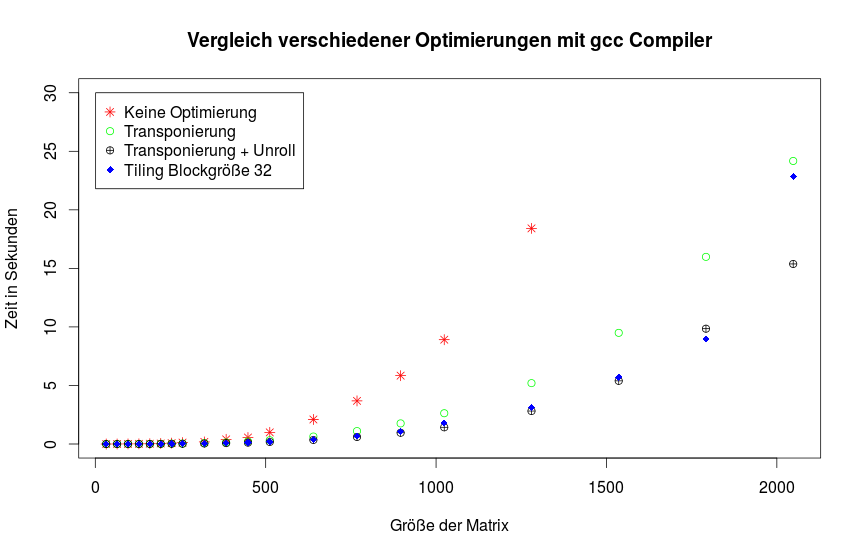
\includegraphics[scale = 0.45]{Bilder/gccO0.png}
\caption{Vergleich der Laufzeiten verschiedener Optimierungen mit dem gcc Compiler. Der Quelltext wurde mit den Parametern -O0 -std=c99 compiliert.}
\noindent\rule{14cm}{0.4pt}
\label{gcc0}
\end{figure}

\begin{figure}[h]
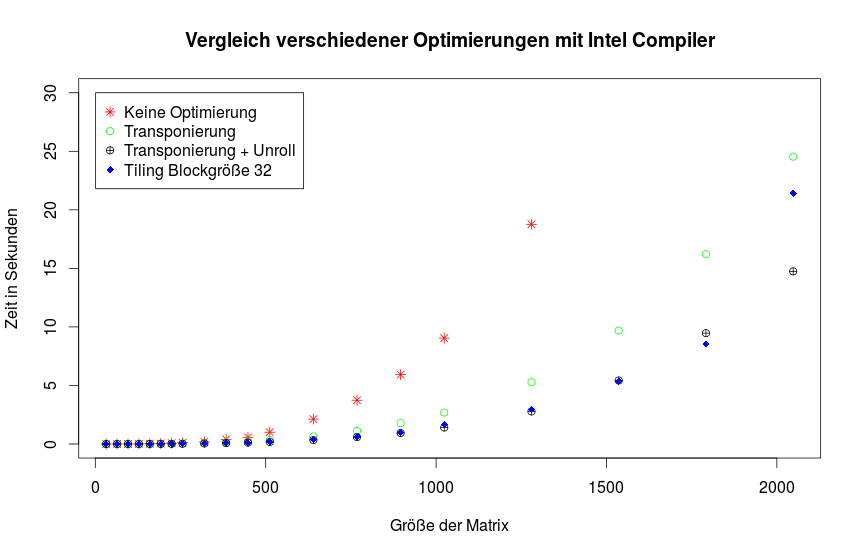
\includegraphics[scale = 0.45]{Bilder/iccO0.png}
\caption{Vergleich der Laufzeiten verschiedener Optimierungen mit dem Intel Compiler. Der Quelltext wurde mit den Parametern -O0 -std=c99 compiliert.}
\noindent\rule{14cm}{0.4pt}
\label{icc0}
\end{figure}

\begin{figure}[h]
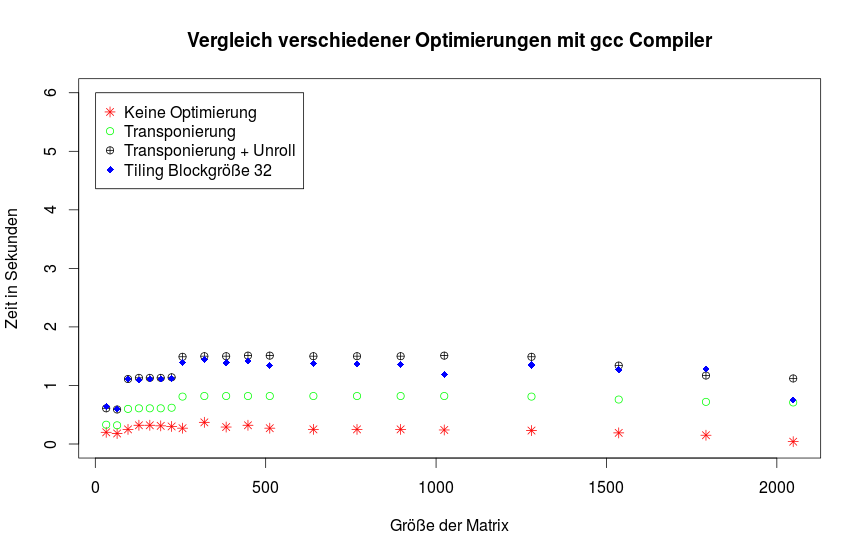
\includegraphics[scale = 0.45]{Bilder/GggcO0.png}
\caption{Vergleich der GFLOP/s verschiedener Optimierungen mit dem gcc Compiler. Der Quelltext wurde mit den Parametern -O0 -std=c99 compiliert.}
\noindent\rule{14cm}{0.4pt}
\label{Ggcc0}
\end{figure}

\begin{figure}[h]
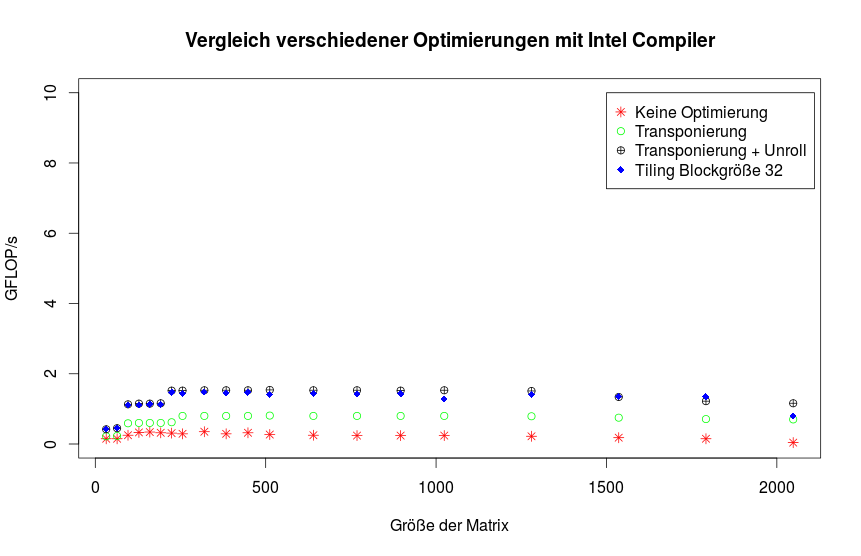
\includegraphics[scale = 0.45]{Bilder/GiccO0.png}
\caption{Vergleich der GFLOP/s verschiedener Optimierungen mit dem Intel Compiler. Der Quelltext wurde mit den Parametern -O0 -std=c99 compiliert.}
\noindent\rule{14cm}{0.4pt}
\label{Gicc0}
\end{figure}

\chapter{Aufgabe 3}
\textit{Überprüfen Sie,  welche  ihrer  manuell  durch geführten  Optimierungen durch  den Einsatz  geeigneter  Compiler-Flags  bzw.  Optimierungsstufen  auch  vom  Compiler realisiert werden.} \newline

Als Compiler Flags haben wir $-O1$, $-O2$ und $-O3$ ausprobiert. Zuerst betrachten wir den gcc Compiler. Die Ausführzeiten für den gcc Compiler sind in den Abbildungen \ref{gccO1}, \ref{gccO2} und \ref{gccO3} gezeigt. Die GFLOP/s sind in den Abbildungen \ref{GgccO1}, \ref{GgccO2} und \ref{GgccO3} zusammengefasst. Der mittels $-O1$ compilierte Quelltext ist im Vergleich zum $-O0$ compilierten Quelltext deutlich schneller. Die geringste Steigerung gibt es für den originalen Quelltext. Hier wird die Matrix nur rund 40\% schneller ausgeführt. Die Steigerung, falls die $B$ Matrix vorher transponiert wurde, beträgt ungefähr 325\%. Das Ausrollen des Quelltextes ist 90\% schneller, falls es mit $-O1$ compiliert wird. Das Tiling benötigt ungefähr halb soviel Zeit. 
Die Ausführzeiten zwischen $-O1$, $-O2$ und $-O3$ compilierten Quelltext sind identisch.

Die Zeiten für den Intel Compiler sind in den Abbildungen \ref{iccO1}, \ref{iccO2} und \ref{iccO3} aufgeführt. Die GFLOP/s Performance ist in den Abbildungen \ref{GiccO1}, \ref{GiccO2} und \ref{GiccO3} zusammengefasst. Auf der $-O1$ Stufe ist der Intel Compiler mit dem gcc Compiler vergleichbar. Die Multiplikation und die Transponierung der $B$ Matrix sind gleich schnell. Ein zusätzliches ausrollen der inneren Schleife wird von gcc Compiler besser übersetzt. Der gcc erzeugt rund 15\% schnelleren Code. Bei der Matrixmultiplikation mit Tiling ist der gcc 0.5 GFLOP/s schneller. Das $-O2$ Flag erzeugt einen deutlichen Performancegewinn beim Intel Compiler. Am deutlichsten wird dies am Quelltext der unverändert compiliert wird. Dieser wird 15x schneller ausgeführt, als mit $-O1$ Flag, und erreicht 4.68 GFLOP/s. Die Transponierung der $B$ Matrix ist mit $-O2$ Flag die schnellste Multiplikationsvariante. Diese Variante wird 2,5 mal schneller ausgeführt als mit $-O1$ Flag. Die Unroll variante ist ungefähr doppelt so schnell. Sie ist aber 1,6 GFLOP/s langsamer als die Transpositionierungs Variante. Bei der Blocking Multiplikation gibt es keine Änderung. Zwischen den $-O2$ und $-O3$ compilierten Varianten gibt es nur für die Ausrollung Variante einen Unterschied. Die Ausrollung ist mit $-O3$ Flag, 1,6 GFLOP/s langsamer als die mit $O2$ compilierten. 

Das $-O1$ Flag des gcc Compiler aktiviert eine Vielzahl von Optimierungen. Beispiels weiße versucht $-fforward-propagate$ zwei Anweisungen zu kombinieren und zu vereinfachen. Das Flag $-freorder-blocks$ vertauscht Basisblöcke um die Codelokalität zu erhöhen. Das $-O2$ und das $-O3$ Flag erhöhen die Performance nicht. 
Der Größe unterschied zwischen den Intel Compiler und den gcc Compiler ist die $-O2$ Optimierungsstufe. Auf der Intel Homepage \footnote{\url{https://software.intel.com/en-us/articles/step-by-step-optimizing-with-intel-c-compiler}} steht: 

``This option enables optimizations for speed. This is the generally recommended optimization level. The compiler vectorization is enabled at O2 and higher levels. With this option, the compiler performs some basic loop optimizations, inlining of intrinsic, Intra-file interprocedural optimization, and most common compiler optimization technologies.''

\begin{table}[h]
  \begin{tabular}{l|l|l|l|l|l|l}
  & \multicolumn{3}{c|}{gcc} &                                      \multicolumn{3}{|c}{Intel} \\

                          & -O1    & -O2    & -O3    &  -O1   & -O2    & -O3 \\
                            \hline
  Keine Optimierung       & 6.5820 & 6.5765 & 6.5713 & 6.7796 & 0.4591 & 0.4527\\
  Transponierung          & 0.8771 & 0.8773 & 0.8827 & 0.8768 & 0.3622 & 0.3617\\
  Transponierung + Unroll & 0.7882 & 0.7885 & 0.7764 & 0.8717 & 0.4965 & 0.7891\\
  Blocking Blockgröße 32  & 0.8339 & 0.8369 & 0.8435 & 1.0509 & 1.0386 & 1.0414\\


  \hline
 \end{tabular}
 \caption{Zusammenfassung der Ausführzeiten für eine Multiplikation von zwei Matrizen der Größe 1024. Die Zeiten sind in Sekunden.}
\end{table}

\begin{table}[h]
  \begin{tabular}{l|l|l|l|l|l|l}
  & \multicolumn{3}{c|}{gcc} &                                      \multicolumn{3}{|c}{Intel} \\

                          & -O1    & -O2    & -O3    &  -O1   & -O2    & -O3 \\
                            \hline
  Keine Optimierung       & 0.33   & 0.33   & 0.33   &  0.29  & 4.68   & 4.74 \\
  Transponierung          & 2.45   & 2.45   & 2.43   &  2.34  & 5.93   & 5.94 \\
  Transponierung + Unroll & 2.72   & 2.72   & 2.77   &  2.43  & 4.33   & 2.72 \\
  Blocking Blockgröße 32  & 2.58   & 2.57   & 2.55   &  2.72  & 2.07   & 2.06 \\

  \hline
 \end{tabular}
  \caption{Zusammenfassung der GFLOP/s für eine Multiplikation von zwei Matrizen der Größe 1024.}
\end{table}

\begin{figure}[h]
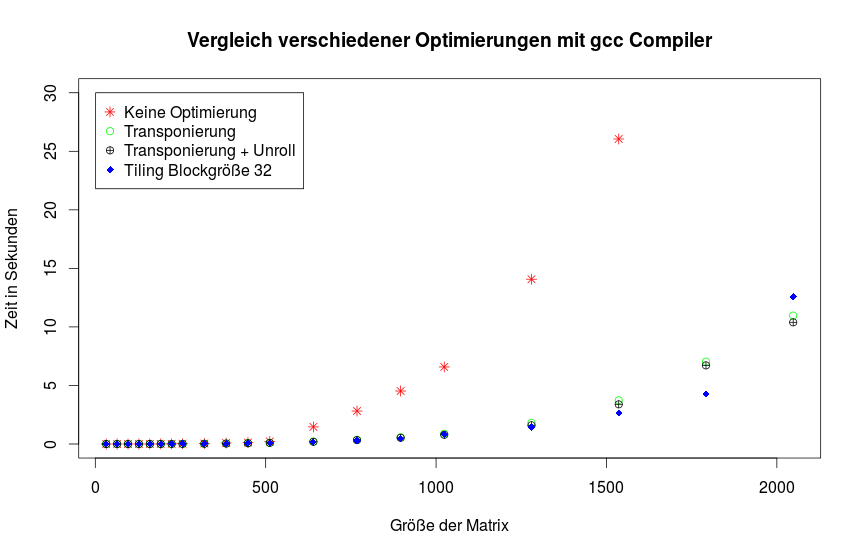
\includegraphics[scale = 0.45]{Bilder/gccO1.png}
\caption{Vergleich der Laufzeiten verschiedener Optimierungen mit dem gcc Compiler. Der Quelltext wurde mit den Parametern -O1 -std=c99 compiliert.}
\noindent\rule{14cm}{0.4pt}
\label{gccO1}
\end{figure}

\begin{figure}[h]
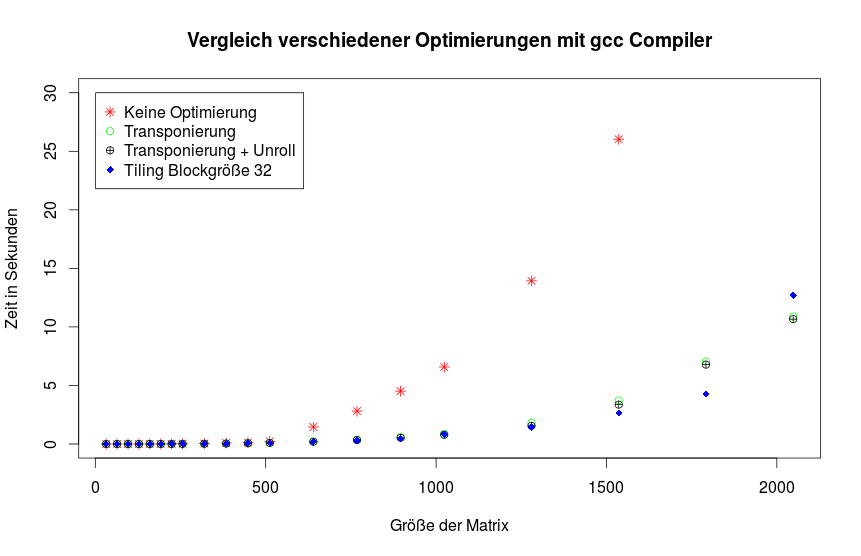
\includegraphics[scale = 0.45]{Bilder/gccO2.png}
\caption{Vergleich der Laufzeiten verschiedener Optimierungen mit dem gcc Compiler. Der Quelltext wurde mit den Parametern -O2 -std=c99 compiliert.}
\noindent\rule{14cm}{0.4pt}
\label{gccO2}
\end{figure}

\begin{figure}[h]
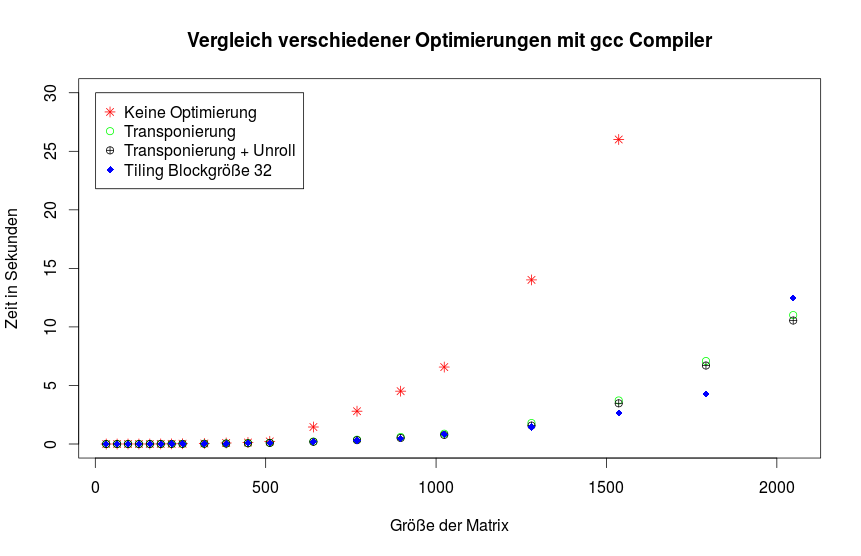
\includegraphics[scale = 0.45]{Bilder/gccO3.png}
\caption{Vergleich der Laufzeiten verschiedener Optimierungen mit dem gcc Compiler. Der Quelltext wurde mit den Parametern -O3 -std=c99 compiliert.}
\noindent\rule{14cm}{0.4pt}
\label{gccO3}
\end{figure}

\begin{figure}[h]
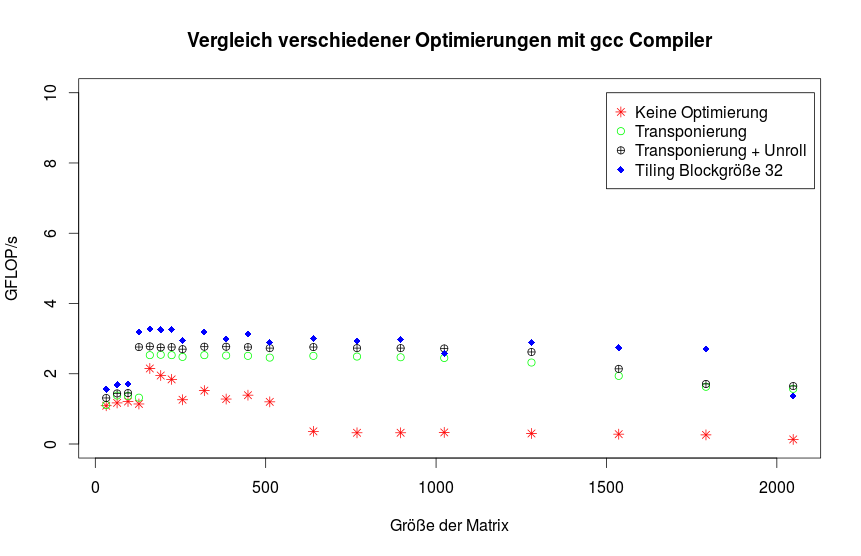
\includegraphics[scale = 0.45]{Bilder/GgccO1.png}
\caption{Vergleich der GFLOP/s verschiedener Optimierungen mit dem gcc Compiler. Der Quelltext wurde mit den Parametern -O1 -std=c99 compiliert.}
\noindent\rule{14cm}{0.4pt}
\label{GgccO1}
\end{figure}

\begin{figure}[h]
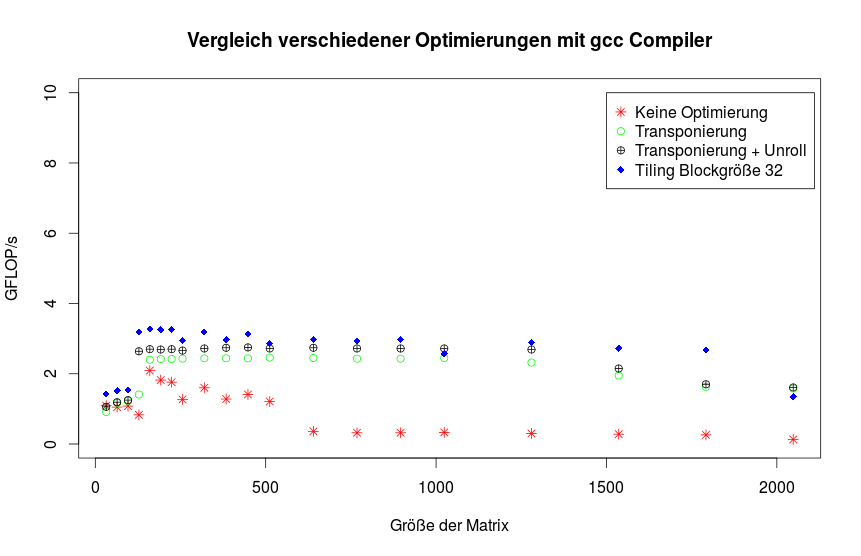
\includegraphics[scale = 0.45]{Bilder/GgccO2.png}
\caption{Vergleich der GFLOP/s verschiedener Optimierungen mit dem gcc Compiler. Der Quelltext wurde mit den Parametern -O2 -std=c99 compiliert.}
\noindent\rule{14cm}{0.4pt}
\label{GgccO2}
\end{figure}

\begin{figure}[h]
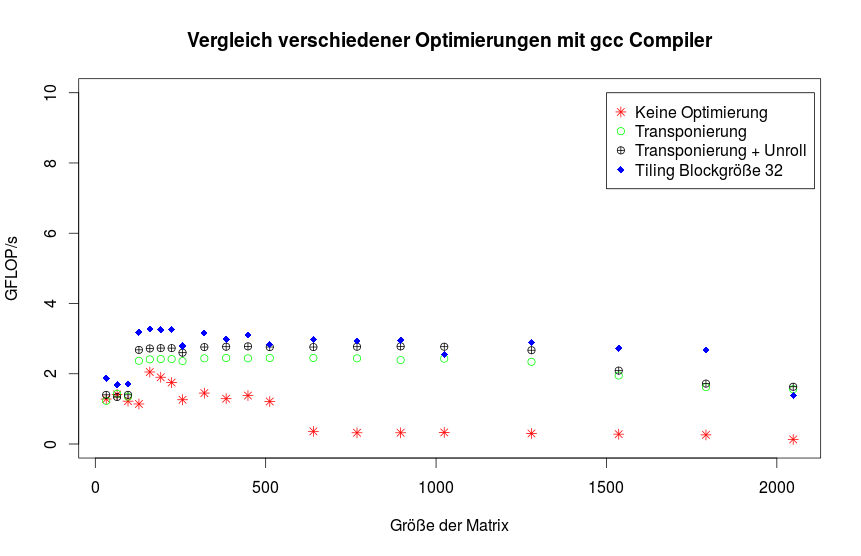
\includegraphics[scale = 0.45]{Bilder/GgccO3.png}
\caption{Vergleich der GFLOP/s verschiedener Optimierungen mit dem gcc Compiler. Der Quelltext wurde mit den Parametern -O3 -std=c99 compiliert.}
\noindent\rule{14cm}{0.4pt}
\label{GgccO3}
\end{figure}

\begin{figure}[h]
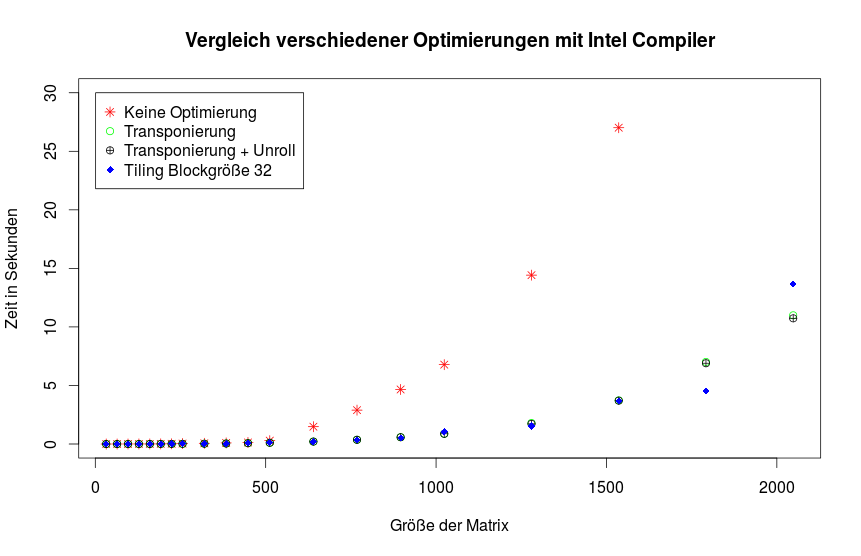
\includegraphics[scale = 0.45]{Bilder/iccO1.png}
\caption{Vergleich der Laufzeiten verschiedener Optimierungen mit dem Intel Compiler. Der Quelltext wurde mit den Parametern -O1 -std=c99 compiliert.}
\noindent\rule{14cm}{0.4pt}
\label{iccO1}
\end{figure}

\begin{figure}[h]
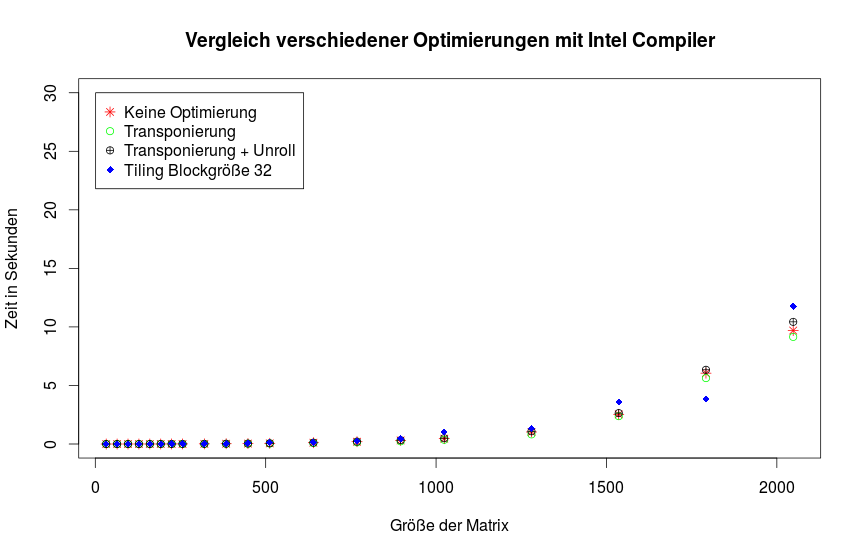
\includegraphics[scale = 0.45]{Bilder/iccO2.png}
\caption{Vergleich der Laufzeiten verschiedener Optimierungen mit dem Intel Compiler. Der Quelltext wurde mit den Parametern -O2 -std=c99 compiliert.}
\noindent\rule{14cm}{0.4pt}
\label{iccO2}
\end{figure}

\begin{figure}[h]
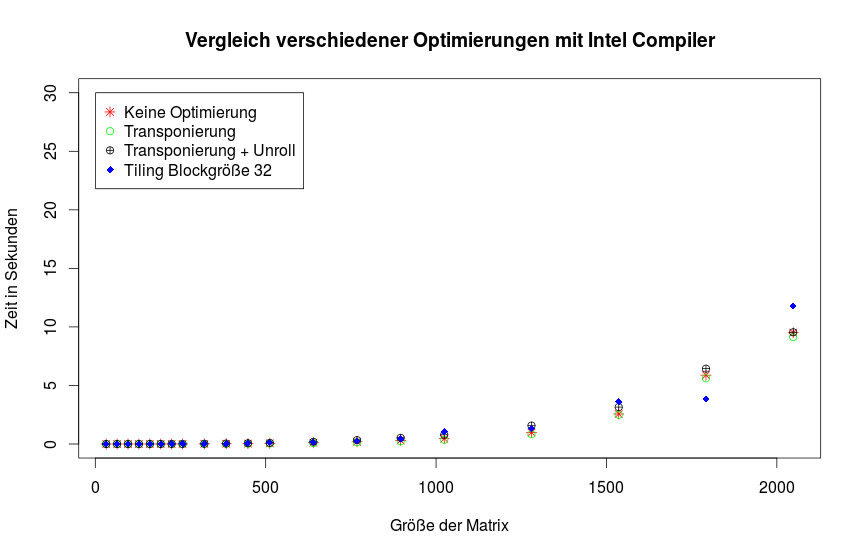
\includegraphics[scale = 0.45]{Bilder/iccO3.png}
\caption{Vergleich der Laufzeiten verschiedener Optimierungen mit dem Intel Compiler. Der Quelltext wurde mit den Parametern -O3 -std=c99 compiliert.}
\noindent\rule{14cm}{0.4pt}
\label{iccO3}
\end{figure}

\begin{figure}[h]
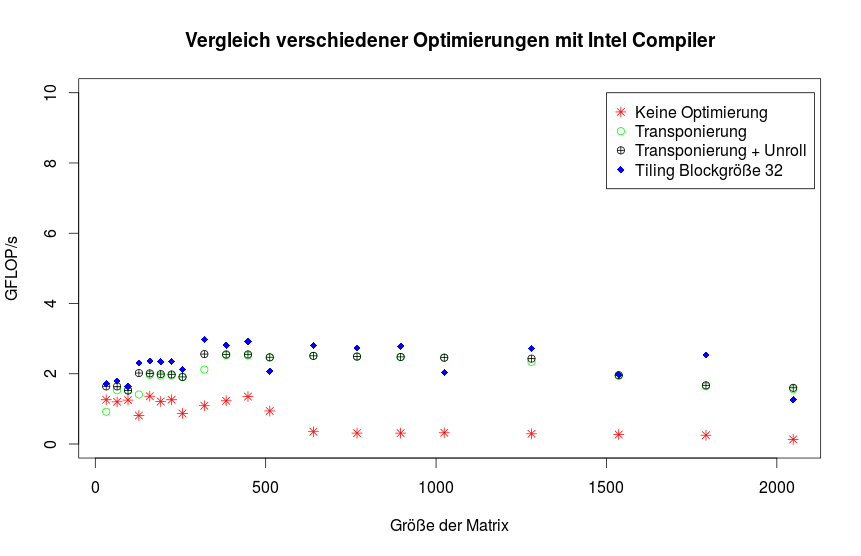
\includegraphics[scale = 0.45]{Bilder/GiccO1.png}
\caption{Vergleich der GFLOP/s verschiedener Optimierungen mit dem Intel Compiler. Der Quelltext wurde mit den Parametern -O1 -std=c99 compiliert.}
\noindent\rule{14cm}{0.4pt}
\label{GiccO1}
\end{figure}

\begin{figure}[h]
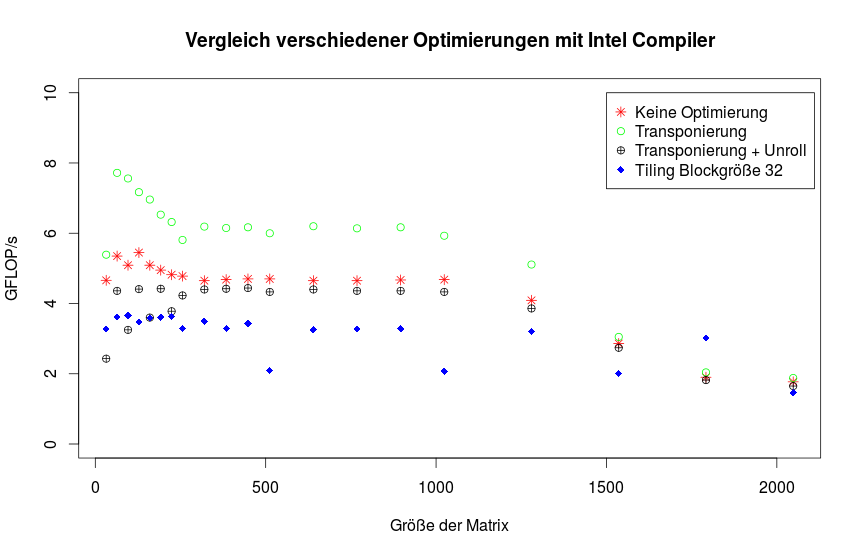
\includegraphics[scale = 0.45]{Bilder/GiccO2.png}
\caption{Vergleich der GFLOP/s verschiedener Optimierungen mit dem Intel Compiler. Der Quelltext wurde mit den Parametern -O2 -std=c99 compiliert.}
\noindent\rule{14cm}{0.4pt}
\label{GiccO2}
\end{figure}

\begin{figure}[h]
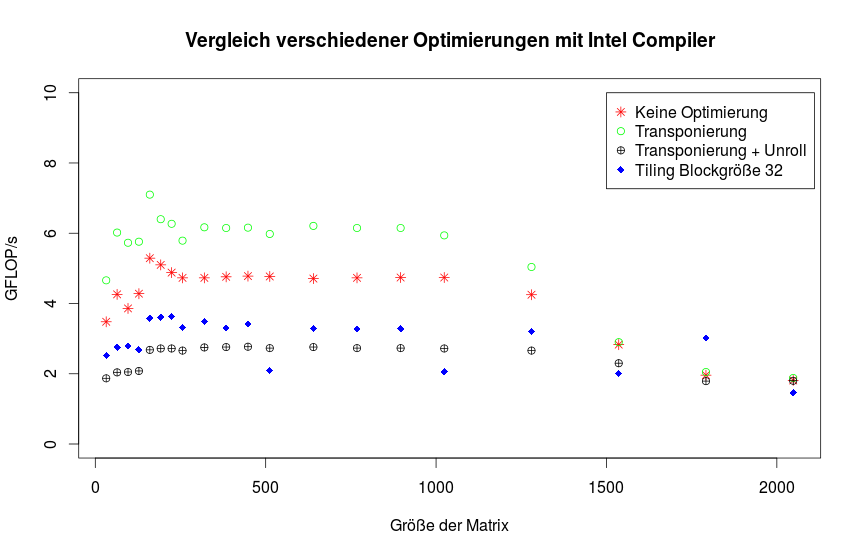
\includegraphics[scale = 0.45]{Bilder/GiccO3.png}
\caption{Vergleich der GFLOP/s verschiedener Optimierungen mit dem Intel Compiler. Der Quelltext wurde mit den Parametern -O3 -std=c99 compiliert.}
\noindent\rule{14cm}{0.4pt}
\label{GiccO3}
\end{figure}


\chapter{Aufgabe 4}
\textit{Berechnen Sie die theoretische Floating-Point-Peak-Performance des Prozessors. Bewerten und begründen Sie die Unterschiede der Leistung ihrer Implementierung im Vergleich zur maximal erreichbaren Leistung.}

Der Intel Xeon E5-2690 hat eine Taktfrequenz von 2,9GHz. Er hat AVX, d.h. er kann 8 single precision Werte Gleichzeitig verarbeiten. Der Sandy Bridge Prozessor besitzt 8 Kerne. Für Single Precision wird Fused multiply add unterstützt.
Die GFLOPS können wie folgt berechnet werden. 
\[2,9 * 8 * 8 * 2 = 371,2 GFLOP/s \]
Im besten Fall erreichen wir Zwei Prozent der maximal möglichen Leistung. Der erste große unterschied der auffällt ist, das wir auf einem Kern statt auf acht rechnen. Der zweite unterschied ist, dass wir Double Precision statt single Presicion benutzen. Hierfür wird Fused multiply add nicht unterstützt. Wir können also eine neue Rechnung aufstellen. Für unser Programm ergibt sich eine maximale Performance von:
\[2,9 * 8 = 23,2 GFLOP/s\]
Die beste Variante erreicht 25\% der Leistung. 

Gründe warum die Leistung in unserer Implementierung niedriger sind, als die theoretische Leistung sind:
\begin{enumerate}
 \item Die $B$ Matrix wird vor und nach der Berechnung transponiert. Dies benötigt quadratisch Zeit, in Bezug auf die Matrixgröße.
 \item Durch die Zählschleifen werden kubisch viele Sprünge durchgeführt.  
 \item Die größeren Matrizen passen nicht in die Caches. Die benötigten Zahlen müssen aus dem Hauptspeicher geladen werden. Dies ist teuer. 
\end{enumerate}



			
\end{document}

















